\documentclass{article} % use larger type; default would be 10pt

\usepackage{pgfplots}
\usetikzlibrary{calc}
\usetikzlibrary{arrows}
\usetikzlibrary{patterns}
\usetikzlibrary{calc,intersections,through,backgrounds}
\usetikzlibrary{decorations.pathreplacing}
        \newcommand\degree[0]{^{\circ}}
        \newcommand\abs[1]{\left|#1\right|}

\title{Play with TikZ}
\author{Just Us}
%\date{} % Activate to display a given date or no date (if empty),
         % otherwise the current date is printed 

\begin{document}
\maketitle

\section{Chap 3 Section 4}






fig-3-4-ex2 graph 

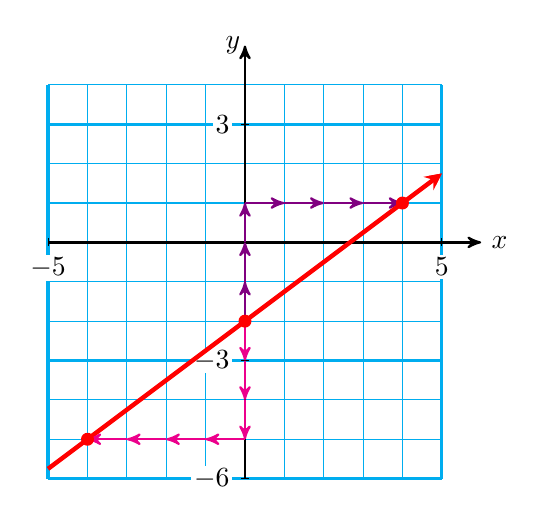
\begin{tikzpicture} [scale=.5]
\draw[cyan] (-5,-6) grid (5,4);
\foreach \x  in  {-5,5} {
 \draw[cyan, very thick] (\x,-6) --++(0,10);
 \draw[black] (\x,0.1) --++(0,-0.2) node[below, yshift=-3, fill=white, inner sep=1]   {$\x$};
}
\foreach \x  in {-6,-3,3} {
 \draw[cyan, very thick] (-5,\x) --++(10,0);
 \draw[black] (.1,\x) --++(-.2,0) node[left, xshift=-3, fill=white, inner sep=1]   {$\x$};
}
\draw[black, thick, ->, >=stealth'] (-5,0)--++(11,0) node[right]{$x$};
\draw[black, thick, ->, >=stealth'] (0,-6)--++(0,11) node[left, xshift=2]{$y$};
\draw[red,  thick, ->,>=stealth] (-5,-23/4)--++(10,15/2);
\foreach \x in {-2,-1,0} 
 \draw[violet,thick,->,>=stealth'] (0,\x)--++(0,1);
\foreach \x in {0,1,2,3} 
 \draw[violet,thick,->,>=stealth'] (\x,1)--++(1,0);
\draw[red, ultra thick, ->,>=stealth] (-5,-23/4)--++(10,15/2);
\foreach \x in {-2,-3,-4} 
 \draw[magenta,thick,->,>=stealth'] (0,\x)--++(0,-1);
\foreach \x in {0,1,2,3} 
 \draw[magenta,thick,->,>=stealth'] (-\x,-5)--++(-1,0);
\filldraw[red] (0,-2) circle (1.5mm);
\filldraw[red] (4,1) circle (1.5mm);
\filldraw[red] (-4,-5) circle (1.5mm);
\end{tikzpicture}
\newline


hp-3-4-5 10-by-10 grid

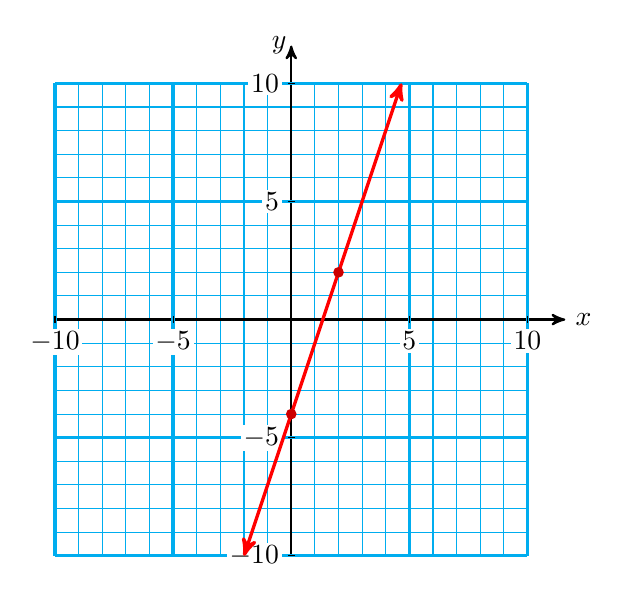
\begin{tikzpicture} [scale=.3]
\draw[cyan] (-10,-10) grid (10,10);
\draw[black,thick, ->, >=stealth'] (-10,0)--(11.6,0) node[right]{$x$};
\draw[black,thick, ->, >=stealth'] (0,-10)--(0,11.6) node[left, xshift=2]{$y$};
\foreach \x in  {-5, 5, -10, 10} {
 \draw[cyan, very thick] (\x,-10) --++(0,20);
 \draw[cyan, very thick] (-10,\x) --++(20,0);
 \draw[black] (\x,.15) --++(0,-.3)  node[below, yshift=-2, fill=white, inner sep=1]   {$\x$};
 \draw[black] (.15,\x) --++(-.3,0)  node[left, xshift=-2, fill=white, inner sep=1]   {$\x$};
}
\draw[red,very thick, <->, >=stealth'] (-2,-10)--(14/3,10);
\filldraw[red!80!black] (0,-4) circle (2mm);
\filldraw[red!80!black] (2,2) circle (2mm);
\end{tikzpicture}
\newline



hp-3-4-6 10-by-10 grid

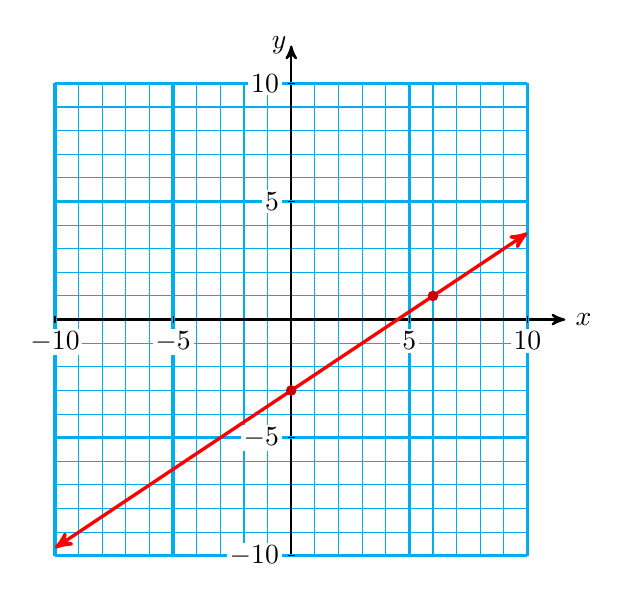
\begin{tikzpicture} [scale=.3]
\draw[cyan] (-10,-10) grid (10,10);
\draw[black,thick, ->, >=stealth'] (-10,0)--(11.6,0) node[right]{$x$};
\draw[black,thick, ->, >=stealth'] (0,-10)--(0,11.6) node[left, xshift=2]{$y$};
\foreach \x in  {-5, 5, -10, 10} {
 \draw[cyan, very thick] (\x,-10) --++(0,20);
 \draw[cyan, very thick] (-10,\x) --++(20,0);
 \draw[black] (\x,.15) --++(0,-.3)  node[below, yshift=-2, fill=white, inner sep=1]   {$\x$};
 \draw[black] (.15,\x) --++(-.3,0)  node[left, xshift=-2, fill=white, inner sep=1]   {$\x$};
}
\draw[red,very thick, <->, >=stealth'] (-10,-29/3)--(10,11/3);
\filldraw[red!80!black] (0,-3) circle (2mm);
\filldraw[red!80!black] (6,1) circle (2mm);
\end{tikzpicture}
\newline



hp-3-4-7 10-by-10 grid

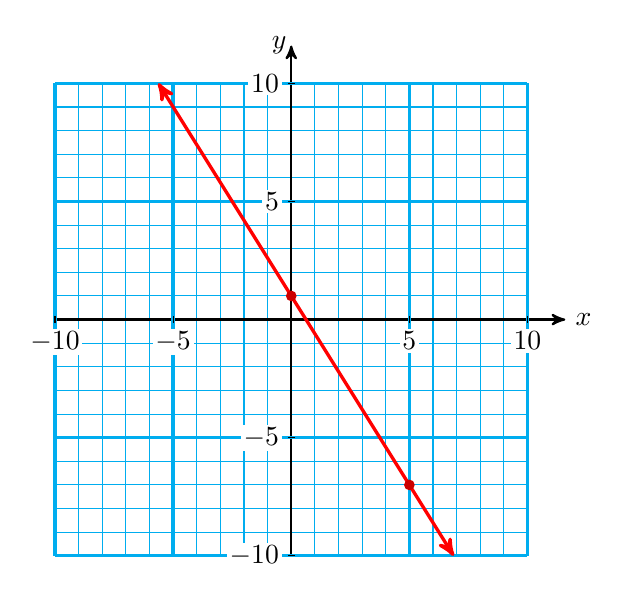
\begin{tikzpicture} [scale=.3]
\draw[cyan] (-10,-10) grid (10,10);
\draw[black,thick, ->, >=stealth'] (-10,0)--(11.6,0) node[right]{$x$};
\draw[black,thick, ->, >=stealth'] (0,-10)--(0,11.6) node[left, xshift=2]{$y$};
\foreach \x in  {-5, 5, -10, 10} {
 \draw[cyan, very thick] (\x,-10) --++(0,20);
 \draw[cyan, very thick] (-10,\x) --++(20,0);
 \draw[black] (\x,.15) --++(0,-.3)  node[below, yshift=-2, fill=white, inner sep=1]   {$\x$};
 \draw[black] (.15,\x) --++(-.3,0)  node[left, xshift=-2, fill=white, inner sep=1]   {$\x$};
}
\draw[red,very thick, <->, >=stealth'] (-45/8,10)--(55/8,-10);
\filldraw[red!80!black] (0,1) circle (2mm);
\filldraw[red!80!black] (5,-7) circle (2mm);
\end{tikzpicture}
\newline


hp-3-4-8 10-by-10 grid

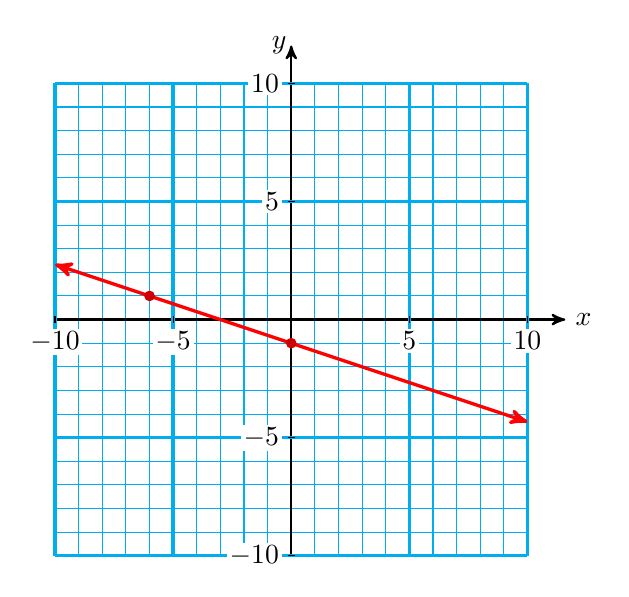
\begin{tikzpicture} [scale=.3]
\draw[cyan] (-10,-10) grid (10,10);
\draw[black,thick, ->, >=stealth'] (-10,0)--(11.6,0) node[right]{$x$};
\draw[black,thick, ->, >=stealth'] (0,-10)--(0,11.6) node[left, xshift=2]{$y$};
\foreach \x in  {-5, 5, -10, 10} {
 \draw[cyan, very thick] (\x,-10) --++(0,20);
 \draw[cyan, very thick] (-10,\x) --++(20,0);
 \draw[black] (\x,.15) --++(0,-.3)  node[below, yshift=-2, fill=white, inner sep=1]   {$\x$};
 \draw[black] (.15,\x) --++(-.3,0)  node[left, xshift=-2, fill=white, inner sep=1]   {$\x$};
}
\draw[red,very thick, <->, >=stealth'] (-10,7/3)--(10,-13/3);
\filldraw[red!80!black] (0,-1) circle (2mm);
\filldraw[red!80!black] (-6,1) circle (2mm);
\end{tikzpicture}
\newline


hp-3-4-8 21

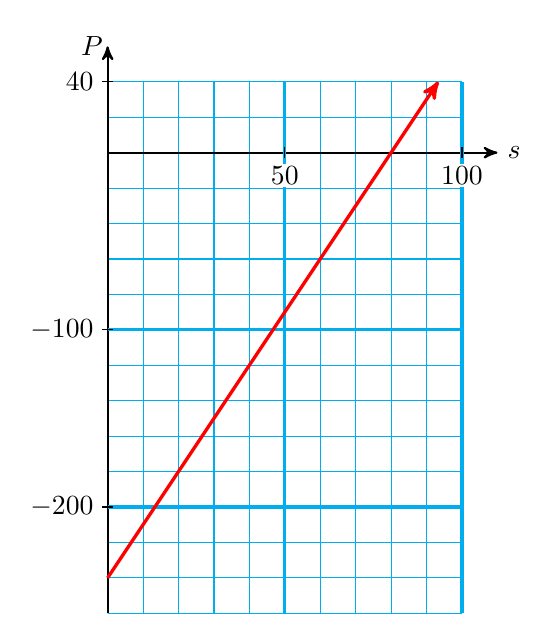
\begin{tikzpicture} [scale=.45]
\draw[cyan] (0,-13) grid (10,2);
\draw[black,thick, ->, >=stealth'] (0,0)--(11,0) node[right]{$s$};
\draw[black,thick, ->, >=stealth'] (0,-13)--(0,3) node[left, xshift=2]{$P$};
\foreach \x [evaluate=\x as \xi using int(10*\x] in  {5, 10} {
 \draw[cyan, very thick] (\x,-13) --++(0,15);
 \draw[black] (\x,.15) --++(0,-.3)  node[below, yshift=-2, fill=white, inner sep=1]   {$\xi$};
}
\foreach \x [evaluate=x as \xi using int(20*\x] in  {-10,-5} {
 \draw[cyan, very thick] (0,\x) --++(10,0);
 \draw[black] (.15,\x) --++(-.3,0)  node[left, xshift=-2, fill=white, inner sep=1]   {$\xi$};
}
\draw[black] (.15,2) --++(-.3,0)  node[left, xshift=-2, fill=white, inner sep=1]   {$40$};
\draw[red,very thick, ->, >=stealth'] (0,-12)--(28/3,2);
\end{tikzpicture}
\newline


hp-3-4-8 22

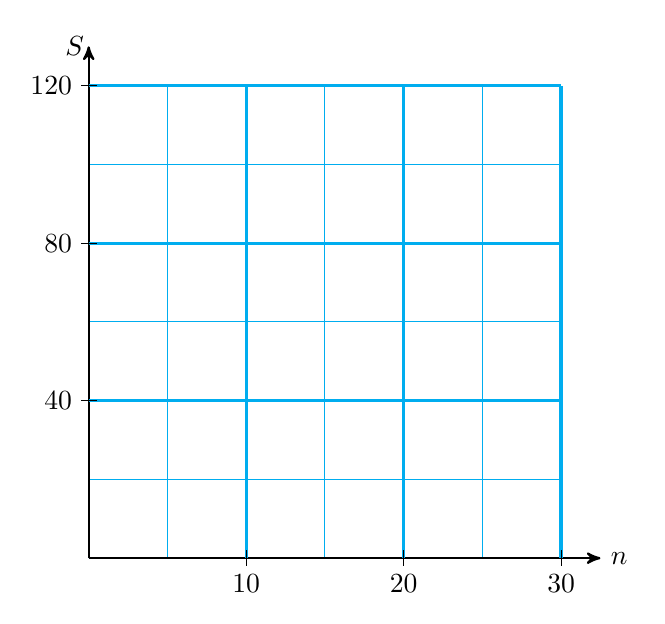
\begin{tikzpicture} 
\draw[cyan] (0,0) grid (6,6);
\draw[black,thick, ->, >=stealth'] (0,0)--(6.5,0) node[right]{$n$};
\draw[black,thick, ->, >=stealth'] (0,0)--(0,6.5) node[left, xshift=2]{$S$};
\foreach \x [evaluate=x as \xi using int(5*\x] in  {2,4,6} {
 \draw[cyan, very thick] (\x,0) --++(0,6);
 \draw[black] (\x,.1) --++(0,-.2)  node[below, yshift=-2, fill=white, inner sep=1]   {$\xi$};
}
\foreach \x [evaluate=x as \xi using int(20*\x] in  {2,4,6} {
 \draw[cyan, very thick] (0,\x) --++(6,0);
 \draw[black] (.1,\x) --++(-.2,0)  node[left, xshift=-2, fill=white, inner sep=1]   {$\xi$};
}
\end{tikzpicture}
\newline


hp-3-4-8 23

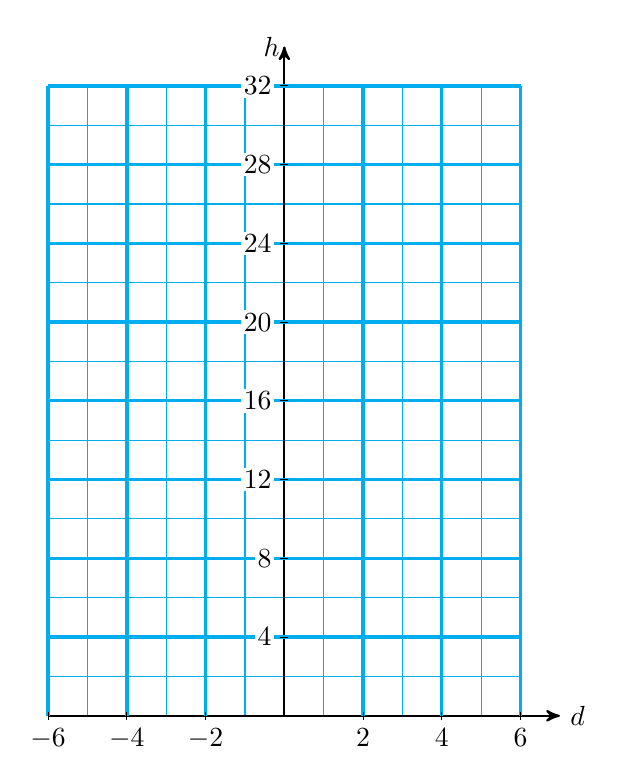
\begin{tikzpicture} [scale=.5]
\draw[cyan] (-6,0) grid (6,16);
\draw[black,thick, ->, >=stealth'] (-6,0)--(7,0) node[right]{$d$};
\draw[black,thick, ->, >=stealth'] (0,0)--(0,17) node[left, xshift=2]{$h$};
\foreach \x in  {-6,-4,-2,2,4,6} {
 \draw[cyan, very thick] (\x,0) --++(0,16);
 \draw[black] (\x,.1) --++(0,-.2)  node[below, yshift=-2, fill=white, inner sep=1]   {$\x$};
}
\foreach \x [evaluate=x as \xi using int(2*\x] in  {2,4,...,16} {
 \draw[cyan, very thick] (-6,\x) --++(12,0);
 \draw[black] (.1,\x) --++(-.2,0)  node[left, xshift=-2, fill=white, inner sep=1]   {$\xi$};
}
\end{tikzpicture}
\newline

hp-3-4-23ans

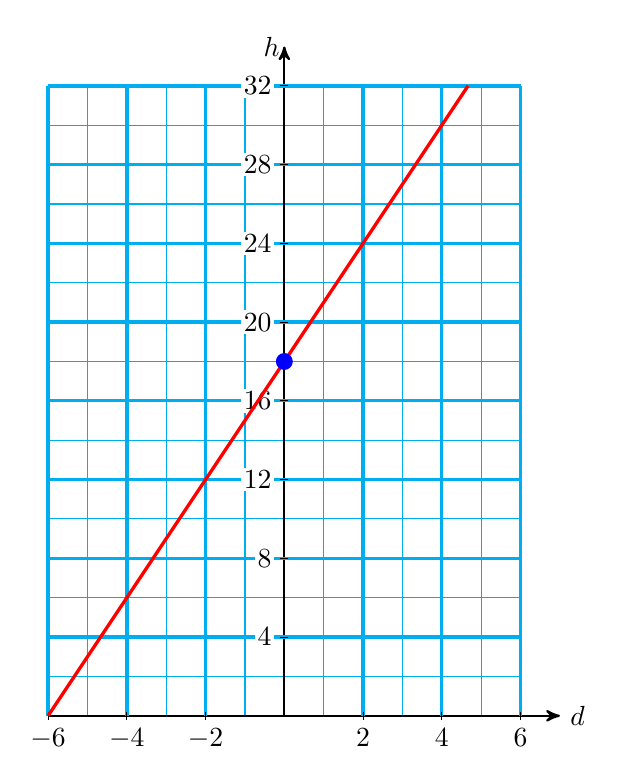
\begin{tikzpicture} [scale=.5]
\draw[cyan] (-6,0) grid (6,16);
\draw[black,thick, ->, >=stealth'] (-6,0)--(7,0) node[right]{$d$};
\draw[black,thick, ->, >=stealth'] (0,0)--(0,17) node[left, xshift=2]{$h$};
\foreach \x in  {-6,-4,-2,2,4,6} {
 \draw[cyan, very thick] (\x,0) --++(0,16);
 \draw[black] (\x,.1) --++(0,-.2)  node[below, yshift=-2, fill=white, inner sep=1]   {$\x$};
}
\foreach \x [evaluate=x as \xi using int(2*\x] in  {2,4,...,16} {
 \draw[cyan, very thick] (-6,\x) --++(12,0);
 \draw[black] (.1,\x) --++(-.2,0)  node[left, xshift=-2, fill=white, inner sep=1]   {$\xi$};
}
\draw[red,very thick] (-6,0)--(14/3,16);
\filldraw[blue] (0,9) circle (2mm);
\end{tikzpicture}
\newline


hp-3-4-8 24

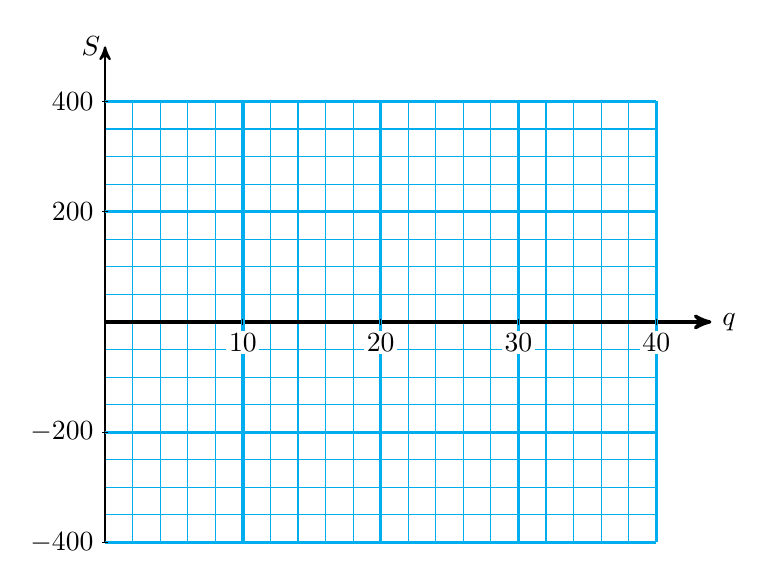
\begin{tikzpicture} [scale=.35]
\draw[cyan] (0,-8) grid (20,8);
\draw[black,very thick, ->, >=stealth'] (0,0)--(22,0) node[right]{$q$};
\draw[black,thick, ->, >=stealth'] (0,-8)--(0,10) node[left, xshift=2]{$S$};
\foreach \x [evaluate=\x as \xi using int(2*\x] in  {5,10,15,20} {
 \draw[cyan, very thick] (\x,-8) --++(0,16);
 \draw[black] (\x,.1) --++(0,-.2)  node[below, yshift=-2, fill=white, inner sep=1]   {$\xi$};
}
\foreach \x [evaluate=x as \xi using int(50*\x] in  {-8,-4,4,8} {
 \draw[cyan, very thick] (0,\x) --++(20,0);
 \draw[black] (.1,\x) --++(-.2,0)  node[left, xshift=-2, fill=white, inner sep=1]   {$\xi$};
}
\end{tikzpicture}
\newline

\section{Chap 3 Section 5}


fig-3-5-1 parallel lines

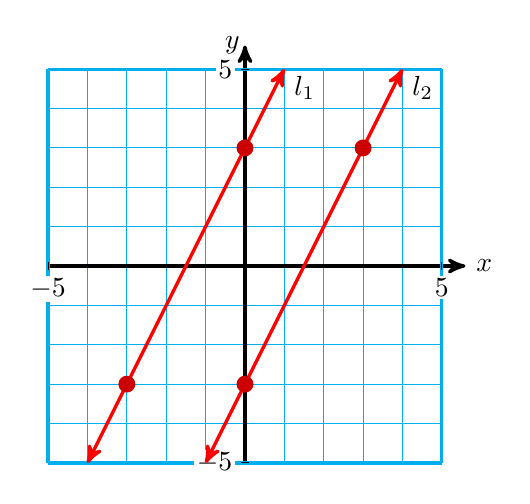
\begin{tikzpicture} [scale=.5]
\draw[cyan] (-5,-5) grid (5,5);
\draw[black,very thick, ->, >=stealth'] (-5,0)--(5.6,0) node[right]{$x$};
\draw[black,very thick, ->, >=stealth'] (0,-5)--(0,5.6) node[left, xshift=2]{$y$};
\foreach \x  in  {-5, 5} {
 \draw[cyan, very thick] (\x,-5) --++(0,10);
 \draw[cyan, very thick] (-5,\x) --++(10,0);
 \draw[black] (\x,.1) --++(0,-.2) node[below, yshift=-2, fill=white, inner sep=1] {$\x$};
 \draw[black] (.1,\x) --++(-.2,0) node[left, xshift=-2, fill=white, inner sep=1]   {$\x$};
}
\draw[red,very thick, <->, >=stealth'] (-4,-5)--(1,5) node[below right, xshift=1, text=black, fill=white, inner sep=2] {$l_1$};
\filldraw[red!80!black] (-3,-3) circle (2mm);
\filldraw[red!80!black] (0,3) circle (2mm);
\draw[red,very thick, <->, >=stealth'] (-1,-5)--(4,5) node[below right, xshift=1, text=black, fill=white, inner sep=2] {$l_2$};
\filldraw[red!80!black] (0,-3) circle (2mm);
\filldraw[red!80!black] (3,3) circle (2mm);
\end{tikzpicture}
\newline


fig-3-5-2 perpendicular lines

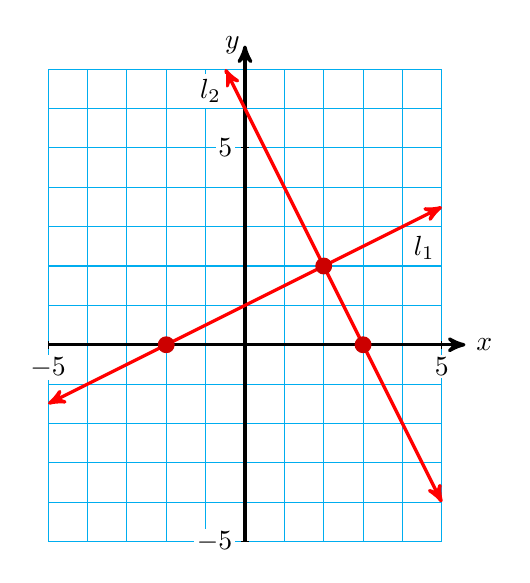
\begin{tikzpicture} [scale=.5]
\draw[cyan] (-5,-5) grid (5,7);
\draw[black,very thick, ->, >=stealth'] (-5,0)--(5.6,0) node[right]{$x$};
\draw[black,very thick, ->, >=stealth'] (0,-5)--(0,7.6) node[left, xshift=2]{$y$};
\foreach \x  in  {-5, 5} {
 \draw[black] (\x,.1) --++(0,-.2) node[below, yshift=-2, fill=white, inner sep=1] {$\x$};
 \draw[black] (.1,\x) --++(-.2,0) node[left, xshift=-2, fill=white, inner sep=1]   {$\x$};
}
\draw[red,very thick, <->, >=stealth'] (-5, -3/2)--(5,7/2) node[below left, yshift=-8, text=black, fill=white, inner sep=2] {$l_1$};
\draw[red,very thick, <->, >=stealth'] (5,-4)--(-1/2,7) node[below left, xshift=1, yshift=-1, text=black, fill=white, inner sep=2] {$l_2$};
\filldraw[red!80!black] (-2,0) circle (2mm);
\filldraw[red!80!black] (2,2) circle (2mm);
\filldraw[red!80!black] (3,0) circle (2mm);
\end{tikzpicture}
\newline

hp-3-3-23 horizontal line
\newline
hp-3-3-24 vertical line
\newline



fig-3-5-ex3 10-by-10 grid

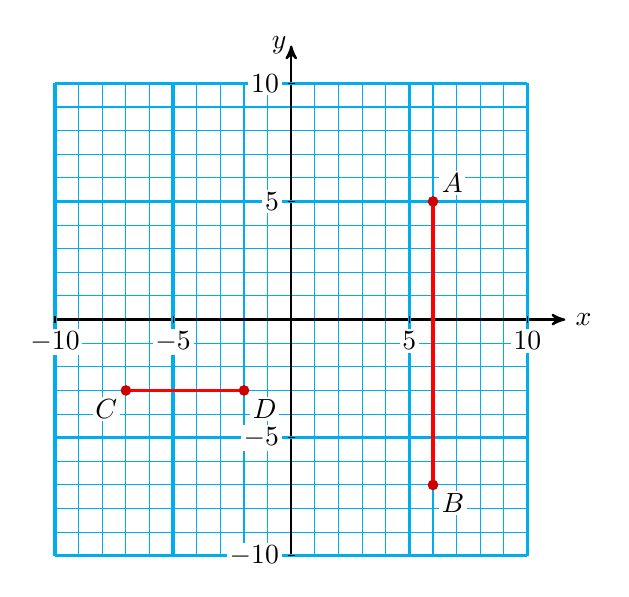
\begin{tikzpicture} [scale=.3]
\draw[cyan] (-10,-10) grid (10,10);
\draw[black,thick, ->, >=stealth'] (-10,0)--(11.6,0) node[right]{$x$};
\draw[black,thick, ->, >=stealth'] (0,-10)--(0,11.6) node[left, xshift=2]{$y$};
\foreach \x in  {-5, 5, -10, 10} {
 \draw[cyan, very thick] (\x,-10) --++(0,20);
 \draw[cyan, very thick] (-10,\x) --++(20,0);
 \draw[black] (\x,.15) --++(0,-.3)  node[below, yshift=-2, fill=white, inner sep=1]   {$\x$};
 \draw[black] (.15,\x) --++(-.3,0)  node[left, xshift=-2, fill=white, inner sep=1]   {$\x$};
}
\coordinate(A) at (6,5);
\coordinate (B) at (6,-7);
\coordinate(C) at (-7,-3);
\coordinate(D) at (-2,-3);
\draw[red,very thick] (A)--(B);
\filldraw[red!80!black] (A) circle (2mm) node[above right, xshift=2, yshift=2, text=black, fill=white, inner sep=1] {$A$};
\filldraw[red!80!black] (B) circle (2mm) node[below right, xshift=2, yshift=-2, text=black, fill=white, inner sep=1] {$B$};
\draw[red,very thick] (C)--(D);
\filldraw[red!80!black] (C) circle (2mm) node[below left, xshift=-2, yshift=-2, text=black, fill=white, inner sep=1] {$C$};
\filldraw[red!80!black] (D) circle (2mm) node[below right, xshift=2, yshift=-2, text=black, fill=white, inner sep=1] {$D$};
\end{tikzpicture}
\newline



fig-3-5-ex4 10-by-10 grid

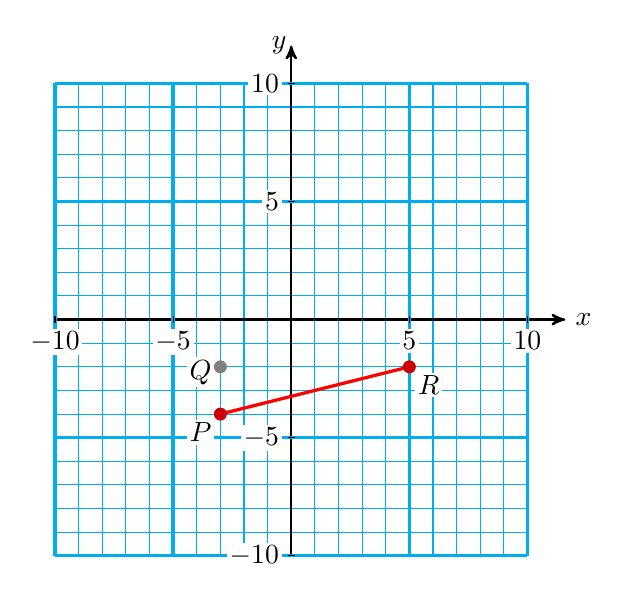
\begin{tikzpicture} [scale=.3]
\draw[cyan] (-10,-10) grid (10,10);
\draw[black,thick, ->, >=stealth'] (-10,0)--(11.6,0) node[right]{$x$};
\draw[black,thick, ->, >=stealth'] (0,-10)--(0,11.6) node[left, xshift=2]{$y$};
\foreach \x in  {-5, 5, -10, 10} {
 \draw[cyan, very thick] (\x,-10) --++(0,20);
 \draw[cyan, very thick] (-10,\x) --++(20,0);
 \draw[black] (\x,.15) --++(0,-.3)  node[below, yshift=-2, fill=white, inner sep=1]   {$\x$};
 \draw[black] (.15,\x) --++(-.3,0)  node[left, xshift=-2, fill=white, inner sep=1]   {$\x$};
}
\coordinate(P) at (-3,-4);
\coordinate (Q) at (-3,-2);
\coordinate(R) at (5,-2);
\draw[red,very thick] (P)--(R);
\filldraw[red!80!black] (P) circle (2.5mm) node[below left, xshift=-2, yshift=-2, text=black, fill=white, inner sep=1] {$P$};
\filldraw[red!80!black] (R) circle (2.5mm) node[below right, xshift=2, yshift=-2, text=black, fill=white, inner sep=1] {$R$};
\filldraw[gray] (Q) circle (2.5mm) node[left, xshift=-2, yshift=-2, text=black, fill=white, inner sep=1] {$Q$};
\end{tikzpicture}
\newline



fig-3-5-ex5 10-by-10 grid

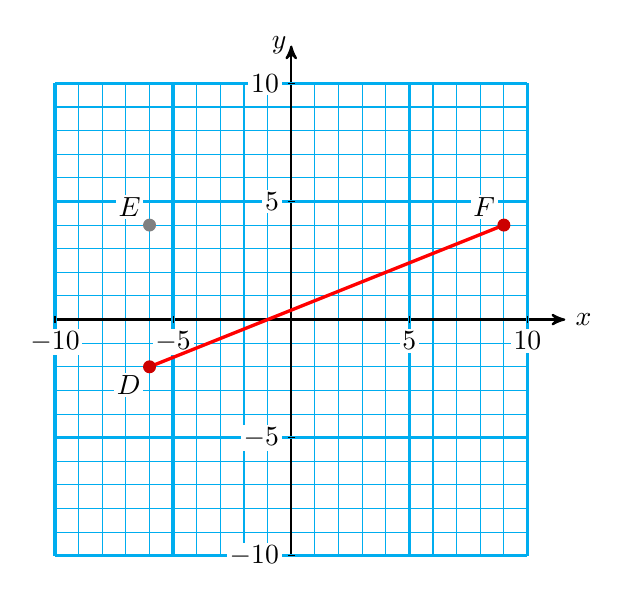
\begin{tikzpicture} [scale=.3]
\draw[cyan] (-10,-10) grid (10,10);
\draw[black,thick, ->, >=stealth'] (-10,0)--(11.6,0) node[right]{$x$};
\draw[black,thick, ->, >=stealth'] (0,-10)--(0,11.6) node[left, xshift=2]{$y$};
\foreach \x in  {-5, 5, -10, 10} {
 \draw[cyan, very thick] (\x,-10) --++(0,20);
 \draw[cyan, very thick] (-10,\x) --++(20,0);
 \draw[black] (\x,.15) --++(0,-.3)  node[below, yshift=-2, fill=white, inner sep=1]   {$\x$};
 \draw[black] (.15,\x) --++(-.3,0)  node[left, xshift=-2, fill=white, inner sep=1]   {$\x$};
}
\coordinate(F) at (9,4);
\coordinate (D) at (-6,-2);
\coordinate(E) at (-6,4);
\draw[red,very thick] (F)--(D);
\filldraw[red!80!black] (F) circle (2.5mm) node[above left, xshift=-2, yshift=2, text=black, fill=white, inner sep=1] {$F$};
\filldraw[red!80!black] (D) circle (2.5mm) node[below left, xshift=-2, yshift=-2, text=black, fill=white, inner sep=1] {$D$};
\filldraw[gray] (E) circle (2.5mm) node[above left, xshift=-2, yshift=2, text=black, fill=white, inner sep=1] {$E$};
\end{tikzpicture}
\newline



hp-3-5-30 

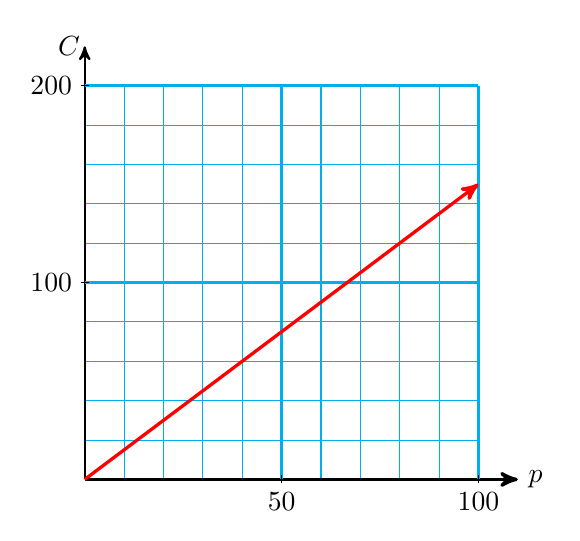
\begin{tikzpicture} [scale=.5]
\draw[cyan] (0,0) grid (10,10);
\draw[black,very thick, ->, >=stealth'] (0,0)--(11,0) node[right]{$p$};
\draw[black,thick, ->, >=stealth'] (0,0)--(0,11) node[left, xshift=2]{$C$};
\foreach \x [evaluate=\x as \xi using int(10*\x] in  {5,10} {
 \draw[cyan, very thick] (\x,0) --++(0,10);
 \draw[black] (\x,.1) --++(0,-.2)  node[below, yshift=-2, fill=white, inner sep=1]   {$\xi$};
}
\foreach \x [evaluate=x as \xi using int(20*\x] in  {5,10} {
 \draw[cyan, very thick] (0,\x) --++(10,0);
 \draw[black] (.1,\x) --++(-.2,0)  node[left, xshift=-2, fill=white, inner sep=1]   {$\xi$};
}
\draw[red, very thick, ->, >=stealth'] (0,0)--(10,15/2);
\end{tikzpicture}
\newline



hp-3-5-301

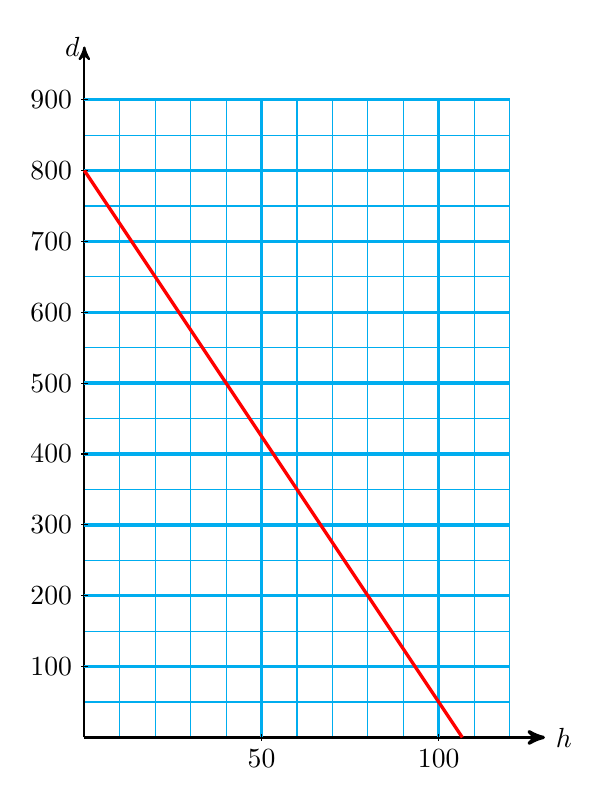
\begin{tikzpicture} [scale=.45]
\draw[cyan] (0,0) grid (12,18);
\draw[black,very thick, ->, >=stealth'] (0,0)--(13,0) node[right]{$h$};
\draw[black,thick, ->, >=stealth'] (0,0)--(0,19.5) node[left, xshift=2]{$d$};
\foreach \x [evaluate=\x as \xi using int(10*\x] in  {5,10} {
 \draw[cyan, very thick] (\x,0) --++(0,18);
 \draw[black] (\x,.1) --++(0,-.2)  node[below, yshift=-2, fill=white, inner sep=1]   {$\xi$};
}
\foreach \x [evaluate=x as \xi using int(50*\x] in  {2,4,...,18} {
 \draw[cyan, very thick] (0,\x) --++(12,0);
 \draw[black] (.1,\x) --++(-.2,0)  node[left, xshift=-2, fill=white, inner sep=1]   {$\xi$};
}
\draw[red, very thick] (0,16)--(32/3,0);
\end{tikzpicture}
\newline



hp-3-5-5ans

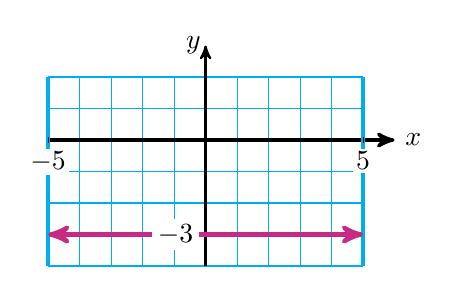
\begin{tikzpicture} [scale=.4]
\draw[cyan] (-5,-4) grid (5,2);
\draw[black,very thick, ->, >=stealth'] (-5,0)--(6,0) node[right]{$x$};
\draw[black,thick, ->, >=stealth'] (0,-4)--(0,3) node[left, xshift=2]{$y$};
\foreach \x  in  {5,-5} {
 \draw[cyan, very thick] (\x,-4) --++(0,6);
 \draw[black] (\x,.1) --++(0,-.2)  node[below, yshift=-2, fill=white, inner sep=1]   {$\x$};
}
\draw[magenta!80!black, ultra thick, <->, >=stealth'] (-5,-3)--(5,-3);
\node[left, fill=white, inner sep=2] at (-.2,-3){$-3$};
\end{tikzpicture}
\newline



hp-3-5-7ans

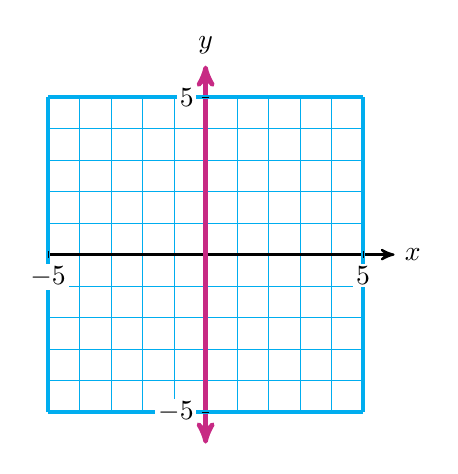
\begin{tikzpicture} [scale=.4]
\draw[cyan] (-5,-5) grid (5,5);
\draw[black, thick, ->, >=stealth'] (-5,0)--(6,0) node[right]{$x$};
\draw[magenta!80!black,ultra thick, <->, >=stealth'] (0,-6)--(0,6) node[above,text=black]{$y$};
\foreach \x  in  {5,-5} {
 \draw[cyan, very thick] (\x,-5) --++(0,10);
 \draw[black] (\x,.1) --++(0,-.2)  node[below, yshift=-2, fill=white, inner sep=1]   {$\x$};
 \draw[cyan, very thick] (-5,\x) --++(10,0);
 \draw[black] (.1,\x) --++(-.2,0)  node[left, xshift=-2, fill=white, inner sep=1]   {$\x$};
}
\end{tikzpicture}
\newline






\section{Chap 3 Review}


cr3-1ans

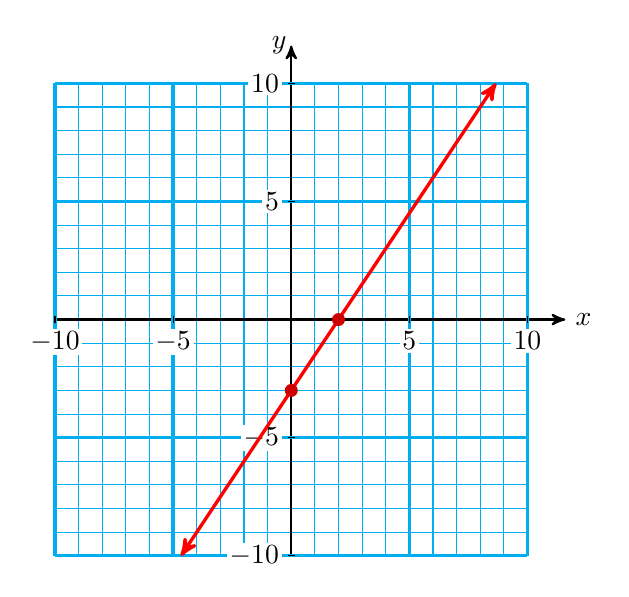
\begin{tikzpicture} [scale=.3]
\draw[cyan] (-10,-10) grid (10,10);
\draw[black,thick, ->, >=stealth'] (-10,0)--(11.6,0) node[right]{$x$};
\draw[black,thick, ->, >=stealth'] (0,-10)--(0,11.6) node[left, xshift=2]{$y$};
\foreach \x in  {-5, 5, -10, 10} {
 \draw[cyan, very thick] (\x,-10) --++(0,20);
 \draw[cyan, very thick] (-10,\x) --++(20,0);
 \draw[black] (\x,.15) --++(0,-.3)  node[below, yshift=-2, fill=white, inner sep=1]   {$\x$};
 \draw[black] (.15,\x) --++(-.3,0)  node[left, xshift=-2, fill=white, inner sep=1]   {$\x$};
}
\coordinate(F) at (0,-3);
\coordinate (D) at (2,0);
\draw[red,very thick, <->, >=stealth'] (-14/3,-10)--(26/3,10);
\filldraw[red!80!black] (F) circle (2.5mm);
\filldraw[red!80!black] (D) circle (2.5mm);
\end{tikzpicture}
\newline


cr3-17 10-by-10 grid

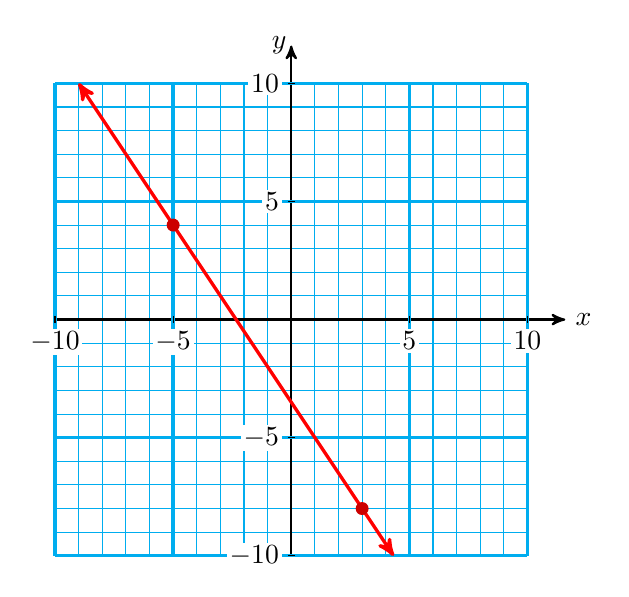
\begin{tikzpicture} [scale=.3]
\draw[cyan] (-10,-10) grid (10,10);
\draw[black,thick, ->, >=stealth'] (-10,0)--(11.6,0) node[right]{$x$};
\draw[black,thick, ->, >=stealth'] (0,-10)--(0,11.6) node[left, xshift=2]{$y$};
\foreach \x in  {-5, 5, -10, 10} {
 \draw[cyan, very thick] (\x,-10) --++(0,20);
 \draw[cyan, very thick] (-10,\x) --++(20,0);
 \draw[black] (\x,.15) --++(0,-.3)  node[below, yshift=-2, fill=white, inner sep=1]   {$\x$};
 \draw[black] (.15,\x) --++(-.3,0)  node[left, xshift=-2, fill=white, inner sep=1]   {$\x$};
}
\coordinate(F) at (-5,4);
\coordinate (D) at (3,-8);
\draw[red,very thick, <->, >=stealth'] (-9,10)--(13/3,-10);
\filldraw[red!80!black] (F) circle (2.5mm);
\filldraw[red!80!black] (D) circle (2.5mm);
\end{tikzpicture}
\newline



cr3-18 10-by-10 grid

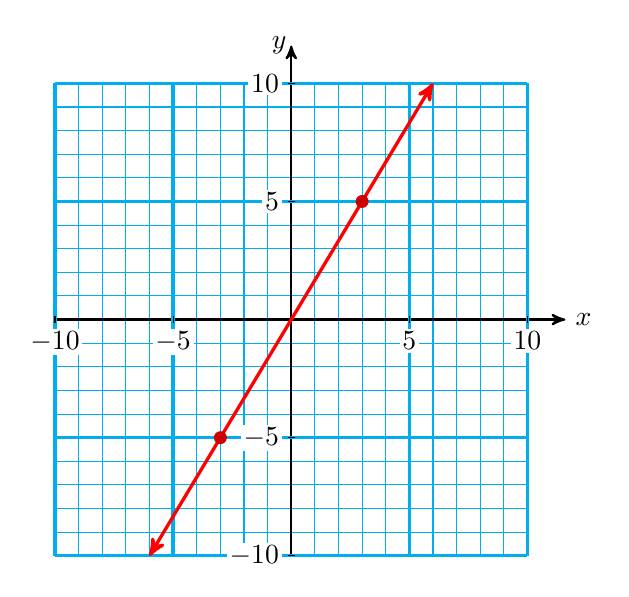
\begin{tikzpicture} [scale=.3]
\draw[cyan] (-10,-10) grid (10,10);
\draw[black,thick, ->, >=stealth'] (-10,0)--(11.6,0) node[right]{$x$};
\draw[black,thick, ->, >=stealth'] (0,-10)--(0,11.6) node[left, xshift=2]{$y$};
\foreach \x in  {-5, 5, -10, 10} {
 \draw[cyan, very thick] (\x,-10) --++(0,20);
 \draw[cyan, very thick] (-10,\x) --++(20,0);
 \draw[black] (\x,.15) --++(0,-.3)  node[below, yshift=-2, fill=white, inner sep=1]   {$\x$};
 \draw[black] (.15,\x) --++(-.3,0)  node[left, xshift=-2, fill=white, inner sep=1]   {$\x$};
}
\coordinate(F) at (-3,-5);
\coordinate (D) at (3,5);
\draw[red,very thick, <->, >=stealth'] (6,10)--(-6,-10);
\filldraw[red!80!black] (F) circle (2.5mm);
\filldraw[red!80!black] (D) circle (2.5mm);
\end{tikzpicture}
\newline



cr3-21ans

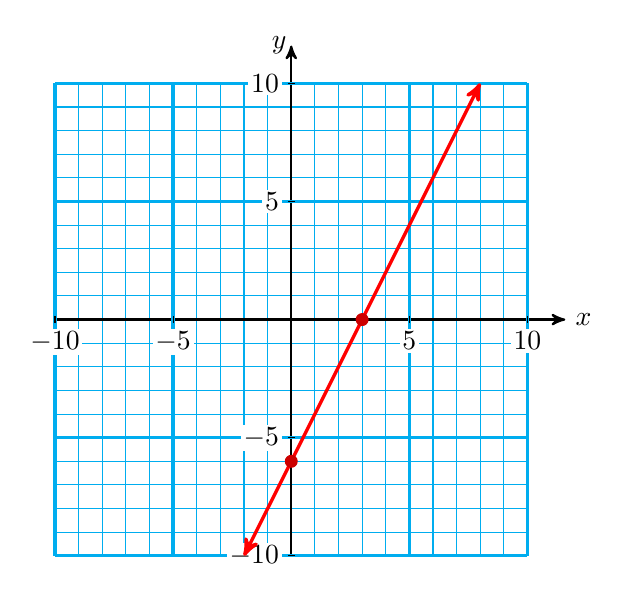
\begin{tikzpicture} [scale=.3]
\draw[cyan] (-10,-10) grid (10,10);
\draw[black,thick, ->, >=stealth'] (-10,0)--(11.6,0) node[right]{$x$};
\draw[black,thick, ->, >=stealth'] (0,-10)--(0,11.6) node[left, xshift=2]{$y$};
\foreach \x in  {-5, 5, -10, 10} {
 \draw[cyan, very thick] (\x,-10) --++(0,20);
 \draw[cyan, very thick] (-10,\x) --++(20,0);
 \draw[black] (\x,.15) --++(0,-.3)  node[below, yshift=-2, fill=white, inner sep=1]   {$\x$};
 \draw[black] (.15,\x) --++(-.3,0)  node[left, xshift=-2, fill=white, inner sep=1]   {$\x$};
}
\coordinate(F) at (3,0);
\coordinate (D) at (0,-6);
\draw[red,very thick, <->, >=stealth'] (8,10)--(-2,-10);
\filldraw[red!80!black] (F) circle (2.5mm);
\filldraw[red!80!black] (D) circle (2.5mm);
\end{tikzpicture}
\newline



cr3-23ans

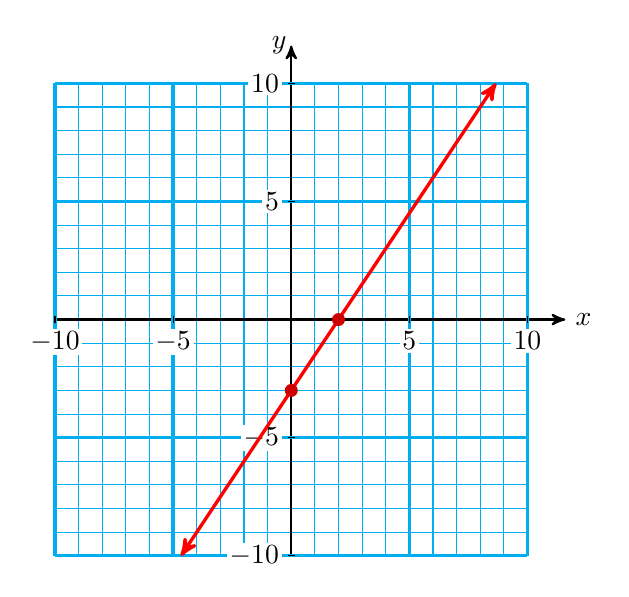
\begin{tikzpicture} [scale=.3]
\draw[cyan] (-10,-10) grid (10,10);
\draw[black,thick, ->, >=stealth'] (-10,0)--(11.6,0) node[right]{$x$};
\draw[black,thick, ->, >=stealth'] (0,-10)--(0,11.6) node[left, xshift=2]{$y$};
\foreach \x in  {-5, 5, -10, 10} {
 \draw[cyan, very thick] (\x,-10) --++(0,20);
 \draw[cyan, very thick] (-10,\x) --++(20,0);
 \draw[black] (\x,.15) --++(0,-.3)  node[below, yshift=-2, fill=white, inner sep=1]   {$\x$};
 \draw[black] (.15,\x) --++(-.3,0)  node[left, xshift=-2, fill=white, inner sep=1]   {$\x$};
}
\coordinate(F) at (2,0);
\coordinate (D) at (0,-3);
\draw[red,very thick, <->, >=stealth'] (-14/3,-10)--(26/3,10);
\filldraw[red!80!black] (F) circle (2.5mm);
\filldraw[red!80!black] (D) circle (2.5mm);
\end{tikzpicture}
\newline



cr3-25 10-by-10 grid

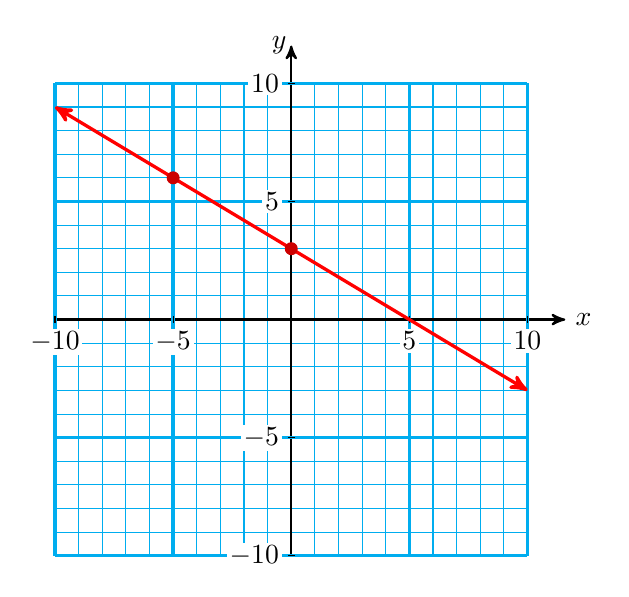
\begin{tikzpicture} [scale=.3]
\draw[cyan] (-10,-10) grid (10,10);
\draw[black,thick, ->, >=stealth'] (-10,0)--(11.6,0) node[right]{$x$};
\draw[black,thick, ->, >=stealth'] (0,-10)--(0,11.6) node[left, xshift=2]{$y$};
\foreach \x in  {-5, 5, -10, 10} {
 \draw[cyan, very thick] (\x,-10) --++(0,20);
 \draw[cyan, very thick] (-10,\x) --++(20,0);
 \draw[black] (\x,.15) --++(0,-.3)  node[below, yshift=-2, fill=white, inner sep=1]   {$\x$};
 \draw[black] (.15,\x) --++(-.3,0)  node[left, xshift=-2, fill=white, inner sep=1]   {$\x$};
}
\coordinate(F) at (-5,6);
\coordinate (D) at (0,3);
\draw[red,very thick, <->, >=stealth'] (-10,9)--(10,-3);
\filldraw[red!80!black] (F) circle (2.5mm);
\filldraw[red!80!black] (D) circle (2.5mm);
\end{tikzpicture}
\newline



cr3-26 10-by-10 grid

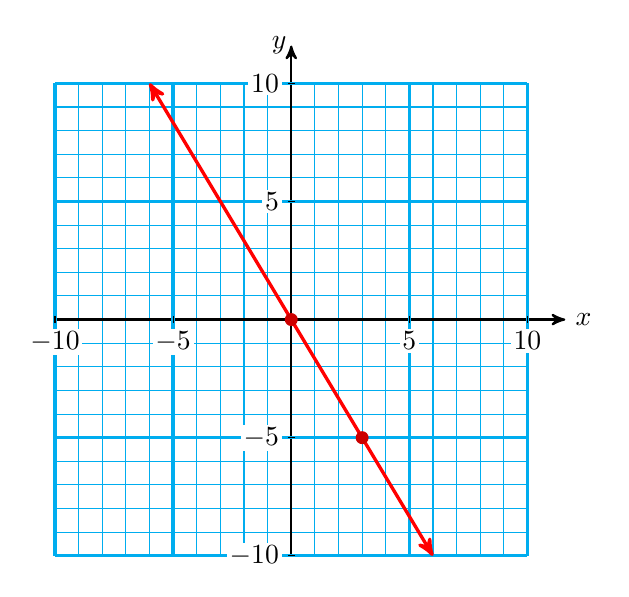
\begin{tikzpicture} [scale=.3]
\draw[cyan] (-10,-10) grid (10,10);
\draw[black,thick, ->, >=stealth'] (-10,0)--(11.6,0) node[right]{$x$};
\draw[black,thick, ->, >=stealth'] (0,-10)--(0,11.6) node[left, xshift=2]{$y$};
\foreach \x in  {-5, 5, -10, 10} {
 \draw[cyan, very thick] (\x,-10) --++(0,20);
 \draw[cyan, very thick] (-10,\x) --++(20,0);
 \draw[black] (\x,.15) --++(0,-.3)  node[below, yshift=-2, fill=white, inner sep=1]   {$\x$};
 \draw[black] (.15,\x) --++(-.3,0)  node[left, xshift=-2, fill=white, inner sep=1]   {$\x$};
}
\coordinate(F) at (0,0);
\coordinate (D) at (3,-5);
\draw[red,very thick, <->, >=stealth'] (-6,10)--(6,-10);
\filldraw[red!80!black] (F) circle (2.5mm);
\filldraw[red!80!black] (D) circle (2.5mm);
\end{tikzpicture}
\newline



cr3-27ans

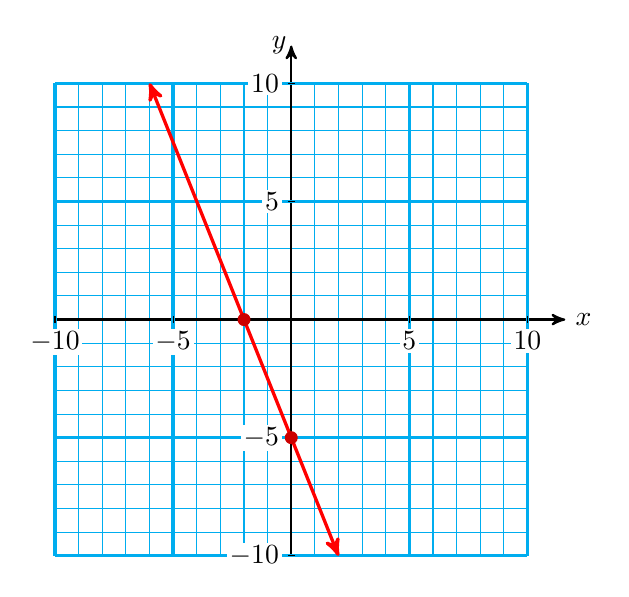
\begin{tikzpicture} [scale=.3]
\draw[cyan] (-10,-10) grid (10,10);
\draw[black,thick, ->, >=stealth'] (-10,0)--(11.6,0) node[right]{$x$};
\draw[black,thick, ->, >=stealth'] (0,-10)--(0,11.6) node[left, xshift=2]{$y$};
\foreach \x in  {-5, 5, -10, 10} {
 \draw[cyan, very thick] (\x,-10) --++(0,20);
 \draw[cyan, very thick] (-10,\x) --++(20,0);
 \draw[black] (\x,.15) --++(0,-.3)  node[below, yshift=-2, fill=white, inner sep=1]   {$\x$};
 \draw[black] (.15,\x) --++(-.3,0)  node[left, xshift=-2, fill=white, inner sep=1]   {$\x$};
}
\coordinate(F) at (-2,0);
\coordinate (D) at (0,-5);
\draw[red,very thick, <->, >=stealth'] (2,-10)--(-6,10);
\filldraw[red!80!black] (F) circle (2.5mm);
\filldraw[red!80!black] (D) circle (2.5mm);
\end{tikzpicture}
\newline



cr3-29ans

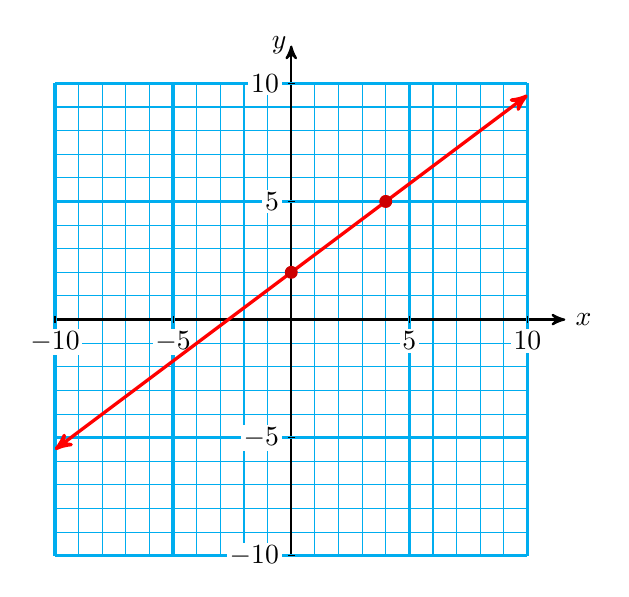
\begin{tikzpicture} [scale=.3]
\draw[cyan] (-10,-10) grid (10,10);
\draw[black,thick, ->, >=stealth'] (-10,0)--(11.6,0) node[right]{$x$};
\draw[black,thick, ->, >=stealth'] (0,-10)--(0,11.6) node[left, xshift=2]{$y$};
\foreach \x in  {-5, 5, -10, 10} {
 \draw[cyan, very thick] (\x,-10) --++(0,20);
 \draw[cyan, very thick] (-10,\x) --++(20,0);
 \draw[black] (\x,.15) --++(0,-.3)  node[below, yshift=-2, fill=white, inner sep=1]   {$\x$};
 \draw[black] (.15,\x) --++(-.3,0)  node[left, xshift=-2, fill=white, inner sep=1]   {$\x$};
}
\coordinate(F) at (4,5);
\coordinate (D) at (0,2);
\draw[red,very thick, <->, >=stealth'] (-10,-11/2)--(10,19/2);
\filldraw[red!80!black] (F) circle (2.5mm);
\filldraw[red!80!black] (D) circle (2.5mm);
\end{tikzpicture}
\newline



cr3-35ans

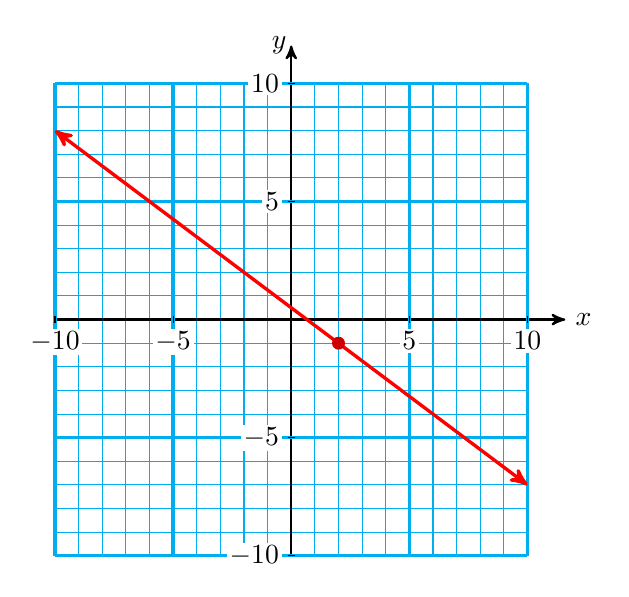
\begin{tikzpicture} [scale=.3]
\draw[cyan] (-10,-10) grid (10,10);
\draw[black,thick, ->, >=stealth'] (-10,0)--(11.6,0) node[right]{$x$};
\draw[black,thick, ->, >=stealth'] (0,-10)--(0,11.6) node[left, xshift=2]{$y$};
\foreach \x in  {-5, 5, -10, 10} {
 \draw[cyan, very thick] (\x,-10) --++(0,20);
 \draw[cyan, very thick] (-10,\x) --++(20,0);
 \draw[black] (\x,.15) --++(0,-.3)  node[below, yshift=-2, fill=white, inner sep=1]   {$\x$};
 \draw[black] (.15,\x) --++(-.3,0)  node[left, xshift=-2, fill=white, inner sep=1]   {$\x$};
}
\coordinate(F) at (2,-1);
\draw[red,very thick, <->, >=stealth'] (-10,8)--(10,-7);
\filldraw[red!80!black] (F) circle (2.5mm);
\end{tikzpicture}
\newline


cr3-51ans

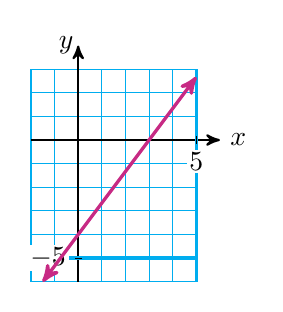
\begin{tikzpicture} [scale=.3]
\draw[cyan] (-2,-6) grid (5,3);
\draw[black,thick, ->, >=stealth'] (-2,0)--(6,0) node[right]{$x$};
\draw[black,thick, ->, >=stealth'] (0,-6)--(0,4) node[left, xshift=2]{$y$};
 \draw[cyan, very thick] (5,-6) --++(0,9);
 \draw[cyan, very thick] (-2,-5) --++(7,0);
 \draw[black] (5,.15) --++(0,-.3)  node[below, yshift=-2, fill=white, inner sep=1]   {$5$};
 \draw[black] (.15,-5) --++(-.3,0)  node[left, xshift=-2, fill=white, inner sep=1]   {$-5$};
\draw[magenta!80!black,very thick, <->, >=stealth'] (-3/2,-6)--(5,8/3);
\end{tikzpicture}
\newline


cr3-53ans

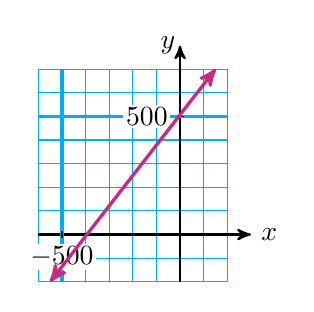
\begin{tikzpicture} [scale=.3]
\draw[cyan] (-6,-2) grid (2,7);
\draw[black,thick, ->, >=stealth'] (-6,0)--(3,0) node[right]{$x$};
\draw[black,thick, ->, >=stealth'] (0,-2)--(0,8) node[left, xshift=2]{$y$};
 \draw[cyan, very thick] (-5,-2) --++(0,9);
 \draw[cyan, very thick] (-6,5) --++(8,0);
 \draw[black] (-5,.15) --++(0,-.3)  node[below, yshift=-2, fill=white, inner sep=1]   {$-500$};
 \draw[black] (.15,5) --++(-.3,0)  node[left, xshift=-2, fill=white, inner sep=1]   {$500$};
\draw[magenta!80!black,very thick, <->, >=stealth'] (-11/2,-2)--(3/2,7);
\end{tikzpicture}
\newline


cr3-55ans

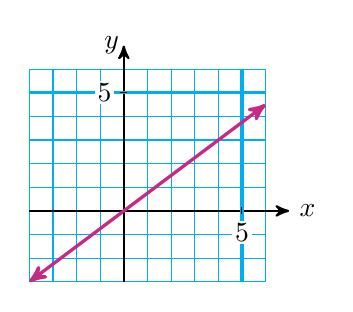
\begin{tikzpicture} [scale=.3]
\draw[cyan] (-4,-3) grid (6,6);
\draw[black,thick, ->, >=stealth'] (-4,0)--(7,0) node[right]{$x$};
\draw[black,thick, ->, >=stealth'] (0,-3)--(0,7) node[left, xshift=2]{$y$};
 \draw[cyan, very thick] (5,-3) --++(0,9);
 \draw[cyan, very thick] (-4,5) --++(10,0);
 \draw[black] (5,.15) --++(0,-.3)  node[below, yshift=-2, fill=white, inner sep=1]   {$5$};
 \draw[black] (.15,5) --++(-.3,0)  node[left, xshift=-2, fill=white, inner sep=1]   {$5$};
\draw[magenta!80!black,very thick, <->, >=stealth'] (-4,-3)--(6,9/2);
\end{tikzpicture}
\newline


cr3-57ans

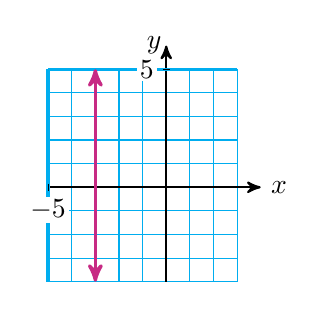
\begin{tikzpicture} [scale=.3]
\draw[cyan] (-5,-4) grid (3,5);
\draw[black,thick, ->, >=stealth'] (-5,0)--(4,0) node[right]{$x$};
\draw[black,thick, ->, >=stealth'] (0,-4)--(0,6) node[left, xshift=2]{$y$};
 \draw[cyan, very thick] (-5,-4) --++(0,9);
 \draw[cyan, very thick] (-5,5) --++(8,0);
 \draw[black] (-5,.15) --++(0,-.3)  node[below, yshift=-2, fill=white, inner sep=1]   {$-5$};
 \draw[black] (.15,5) --++(-.3,0)  node[left, xshift=-2, fill=white, inner sep=1]   {$5$};
\draw[magenta!80!black,very thick, <->, >=stealth'] (-3,-4)--(-3,5);
\end{tikzpicture}
\newline









8 by 8 grid

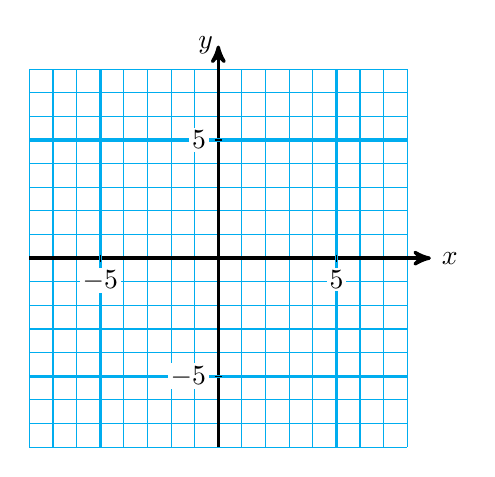
\begin{tikzpicture} [scale=.3]
\draw[cyan] (-8,-8) grid (8,8);
\draw[black,very thick, ->, >=stealth'] (-8,0)--(9,0) node[right]{$x$};
\draw[black,very thick, ->, >=stealth'] (0,-8)--(0,9) node[left, xshift=2]{$y$};
\foreach \x  in  {-5, 5} {
 \draw[cyan, very thick] (\x,-8) --++(0,16);
 \draw[cyan, very thick] (-8,\x) --++(16,0);
 \draw[black] (\x,.15) --++(0,-.3) node[below, yshift=-2, fill=white, inner sep=1]   {$\x$};
 \draw[black] (.15,\x) --++(-.3,0) node[left, xshift=-2, fill=white, inner sep=1]   {$\x$};
}
\end{tikzpicture}
\newline

10 by 10 grid: hp-2-3-12


\end{document}
